% Figure / table inputs

\chapter{Approach and Custom Software solutions}
\todo[inline]{replace CITEME tags in Approach and Custom Software solutions}

\section{Purpose}
Illustrate how lessons learned in previous chapter (as well as new lessons introduced here) are addressed through custom software solutions.
\begin{enumerate}
 \item RNA-seq analysis, reproducibility, updating
 \item Integration of multiple disparate Omics scale data types
 \item Documentation of exactly how analyses were carried out (IPython notebooks)
\end{enumerate}

\todo[inline]{MEGA: you need to write most of this chapter}

\section{The phylogenetic transcriptional correspondence index (PTCI)}








Look at the parameter space of the PTCI (Figure \ref{fig:ptci-space}).  




\begin{figure}[hp]
\centering
  \begin{subfigure}[b]{.9\linewidth}
    \centering

    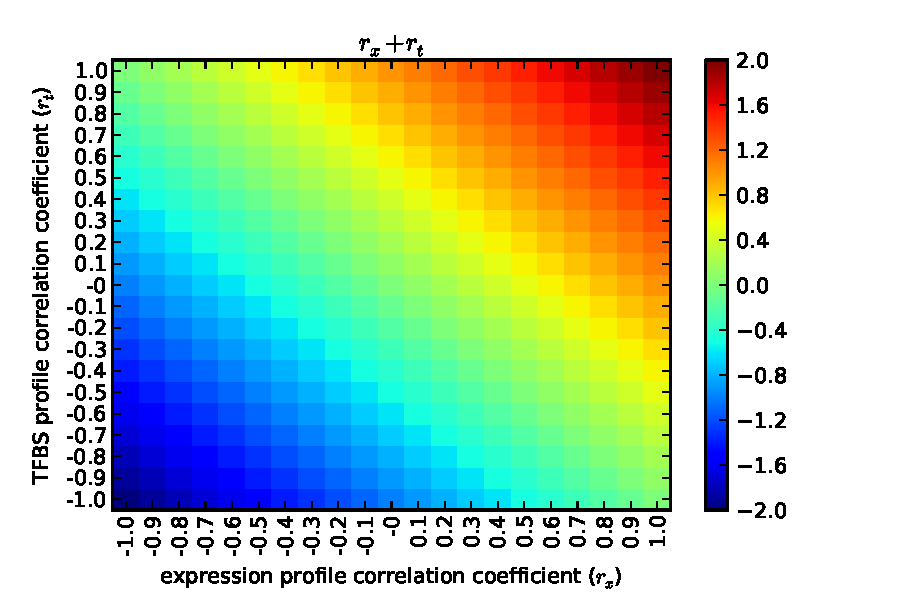
\includegraphics[width=.9\linewidth]{figures/figs/thesis-xprn-tfbs.pdf}
    \caption{}
    \label{fig:ptci-space-a}
  \end{subfigure}%

  

  \begin{subfigure}[b]{.9\linewidth}
    \centering

    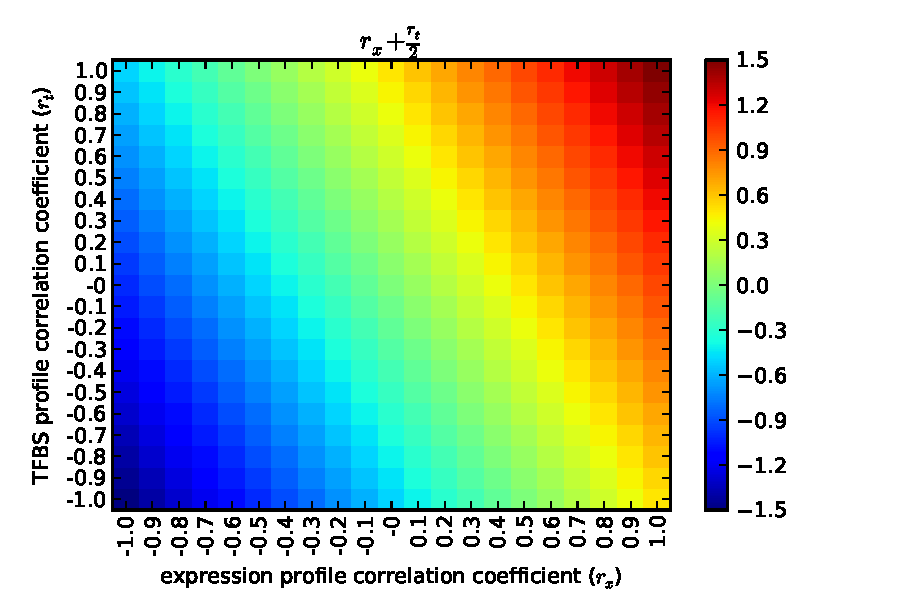
\includegraphics[width=.9\linewidth]{figures/figs/thesis-xprn-scaled-tfbs.pdf}
    \caption{}
    \label{fig:ptci-space-b}
  \end{subfigure}

\caption[Exploring the parameter space of the expression and TFBS components of the PTCI]{\sf \textbf{Exploring the parameter space of the expression and TFBS components of the PTCI:} \\
\textbf{(A)} The expression and TFBS profile correlations each carry the same weight.  TFBS data is not strictly empirical, and position weight matrix models inherently are prone to produce false positive predictions. Here, each correlation-type exerts equal influence on the final score assigned to the ortholog relationship.  \textbf{(B)} The TFBS profile correlation is penalized due to the non-empirical nature and expected false positive information it contains. Here, TFBS profile data contributes to the final score at most 50\% as much as expression data.}
\label{fig:ptci-space}
\end{figure}

Here is the PTCI calculation:


\begin{equation} \label{eq:ptci}
PTCI = ( r_{x} + \frac{r_{t}}{2} ) \cdot w(d)
\end{equation}


The graph model is useful (Figure \ref{fig:nway-ortholog-graph})


\begin{figure}[hp]
\centering
% 
    \begin{subfigure}[t]{.5\linewidth}
    \centering
    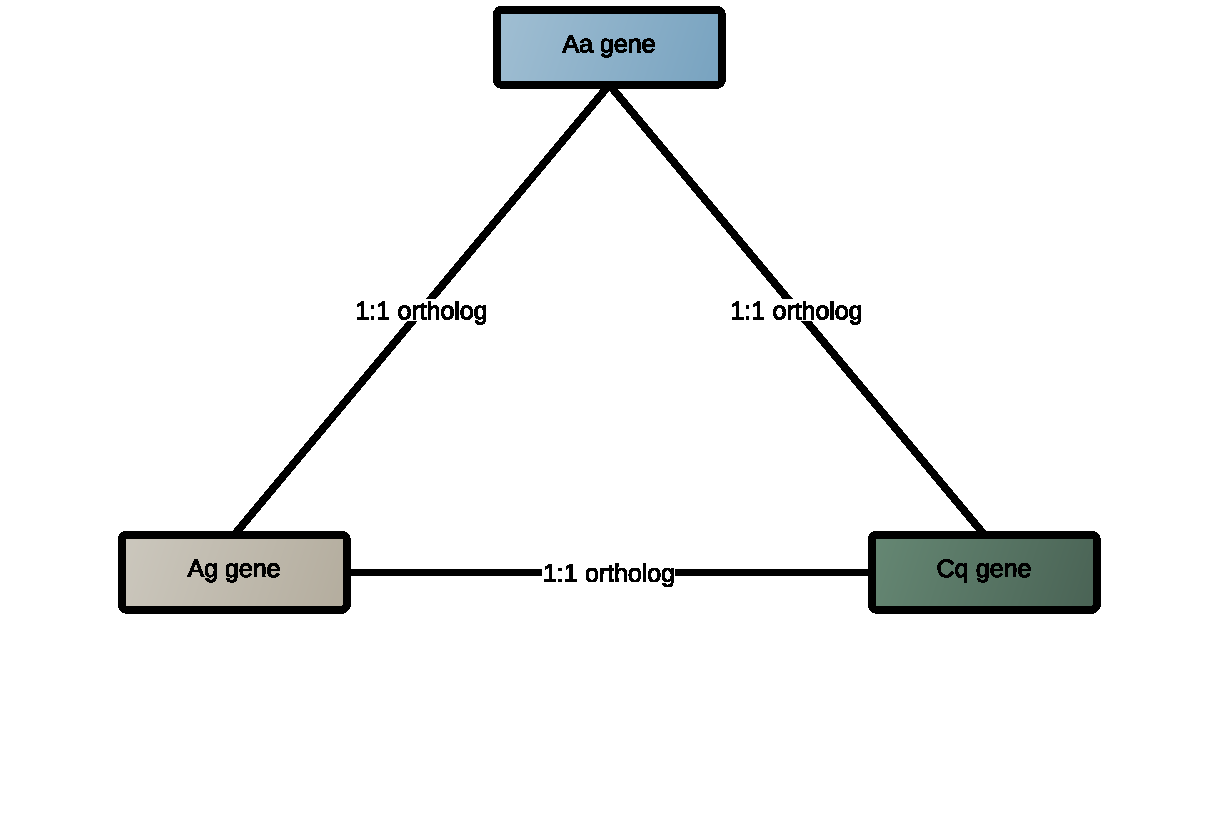
\includegraphics[width=\linewidth]{figures/figs/gfunc_graph_figs/ortho-graph-model.pdf}
    \caption{N-way 1:1 ortholog graph structure}\label{fig:nway-ortholog-graph-model}
    \end{subfigure}%
% 
% 
% 
    \begin{subfigure}[t]{.5\linewidth}
    \centering
    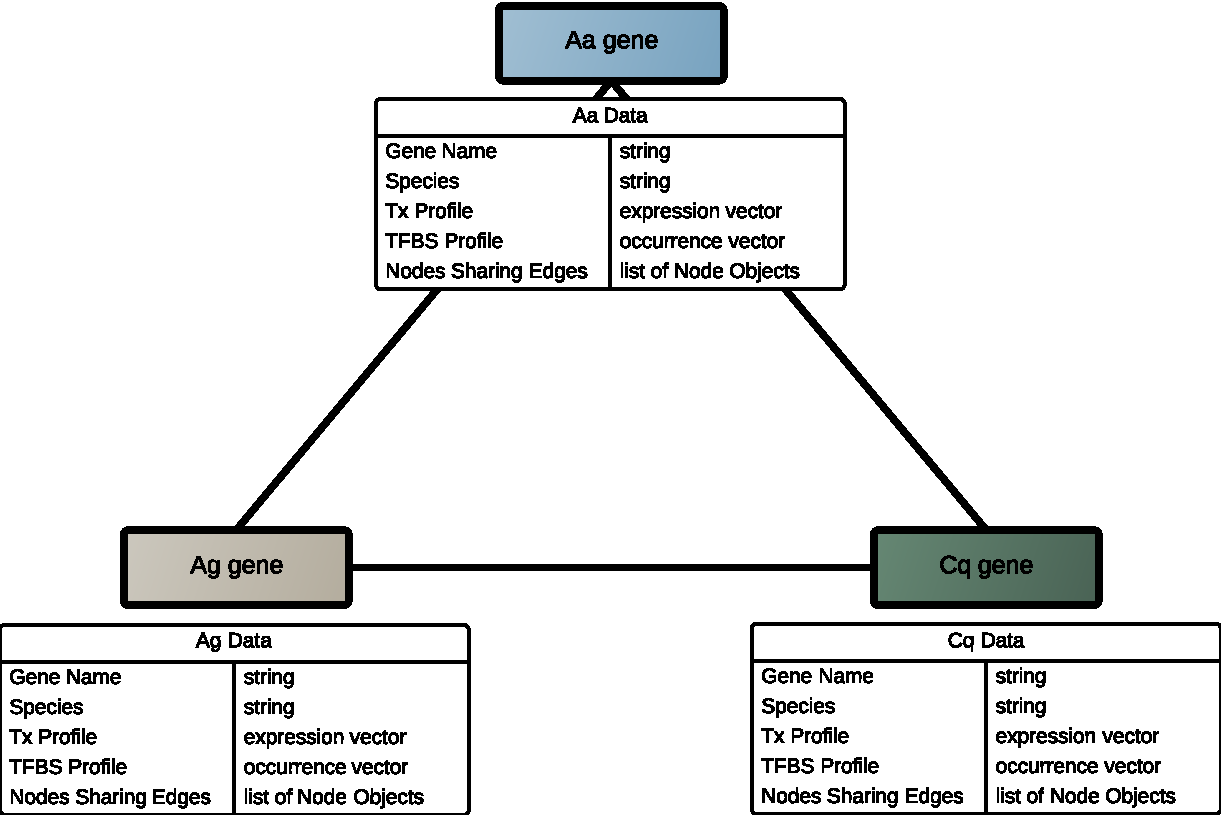
\includegraphics[width=\linewidth]{figures/figs/gfunc_graph_figs/ortho-graph-node-data.pdf}
    \caption{Node data model}\label{fig:nway-ortholog-graph-node-data}
    \end{subfigure}
% 
% 
% 
% 
% 
% 
    \begin{subfigure}[t]{.5\linewidth}
    \centering
    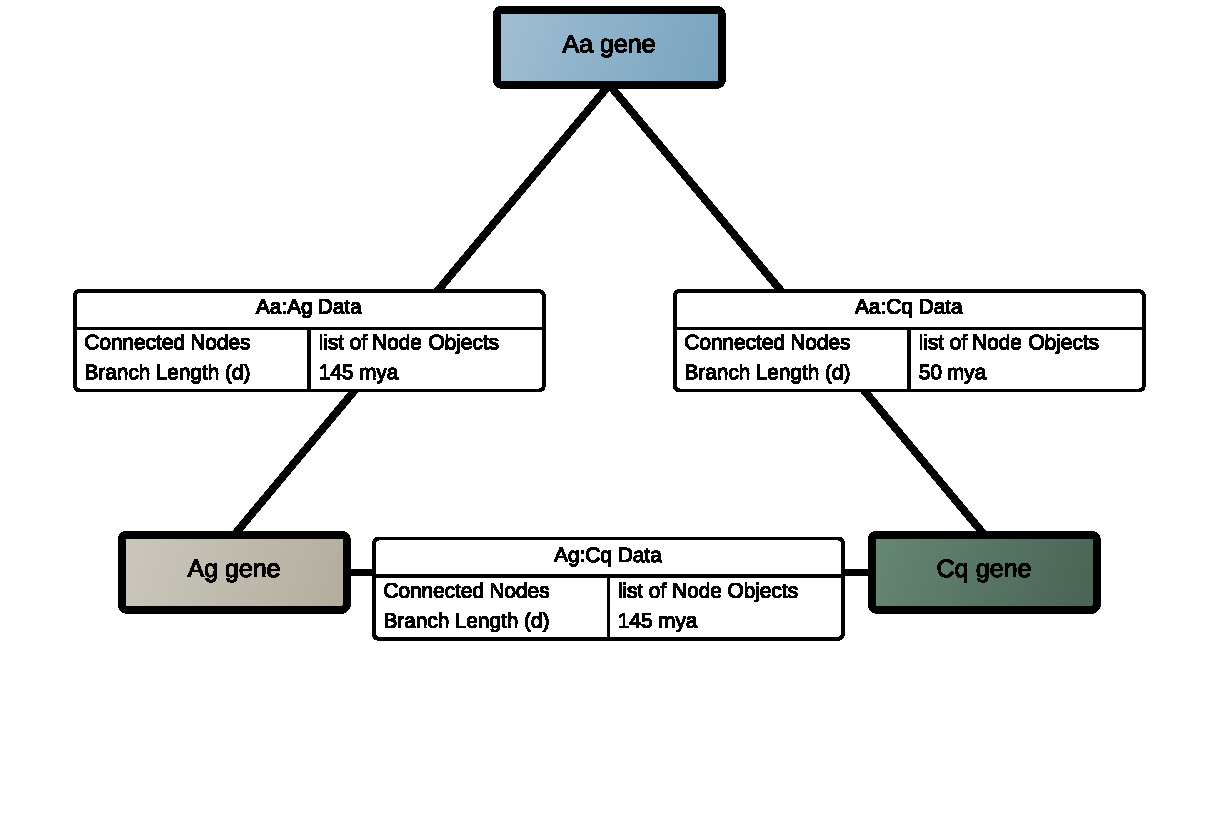
\includegraphics[width=\linewidth]{figures/figs/gfunc_graph_figs/ortho-graph-edge-data.pdf}
    \caption{Edge data model}\label{fig:nway-ortholog-graph-edge-data}
    \end{subfigure}%
% 
% 
%     
    \begin{subfigure}[t]{.5\linewidth}
    \centering
    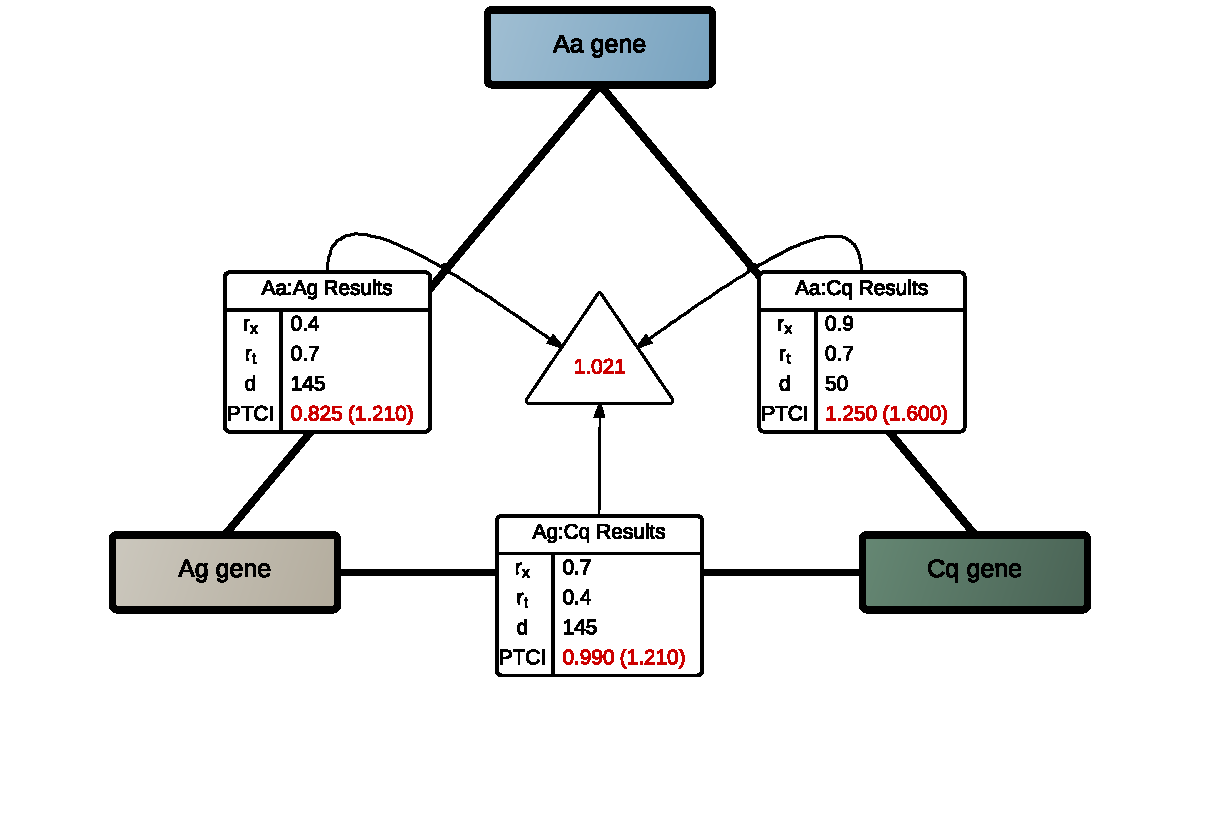
\includegraphics[width=\linewidth]{figures/figs/gfunc_graph_figs/ortho-graph-ptci.pdf}
    \caption{Example PTCI data}\label{fig:nway-ortholog-graph-ptci}
    \end{subfigure}
% 
% 
% 
\caption[Graph model used to integrate data types]{\sf \textbf{Graph model used to integrate data types.}}\label{fig:nway-ortholog-graph}
\end{figure}


\pagebreak[4]
\section{Blacktie RNA-seq pipeline}

See Figure \ref{fig:tuxedo}




\begin{landscape}
 
 
 \begin{figure}[hp]
\centering
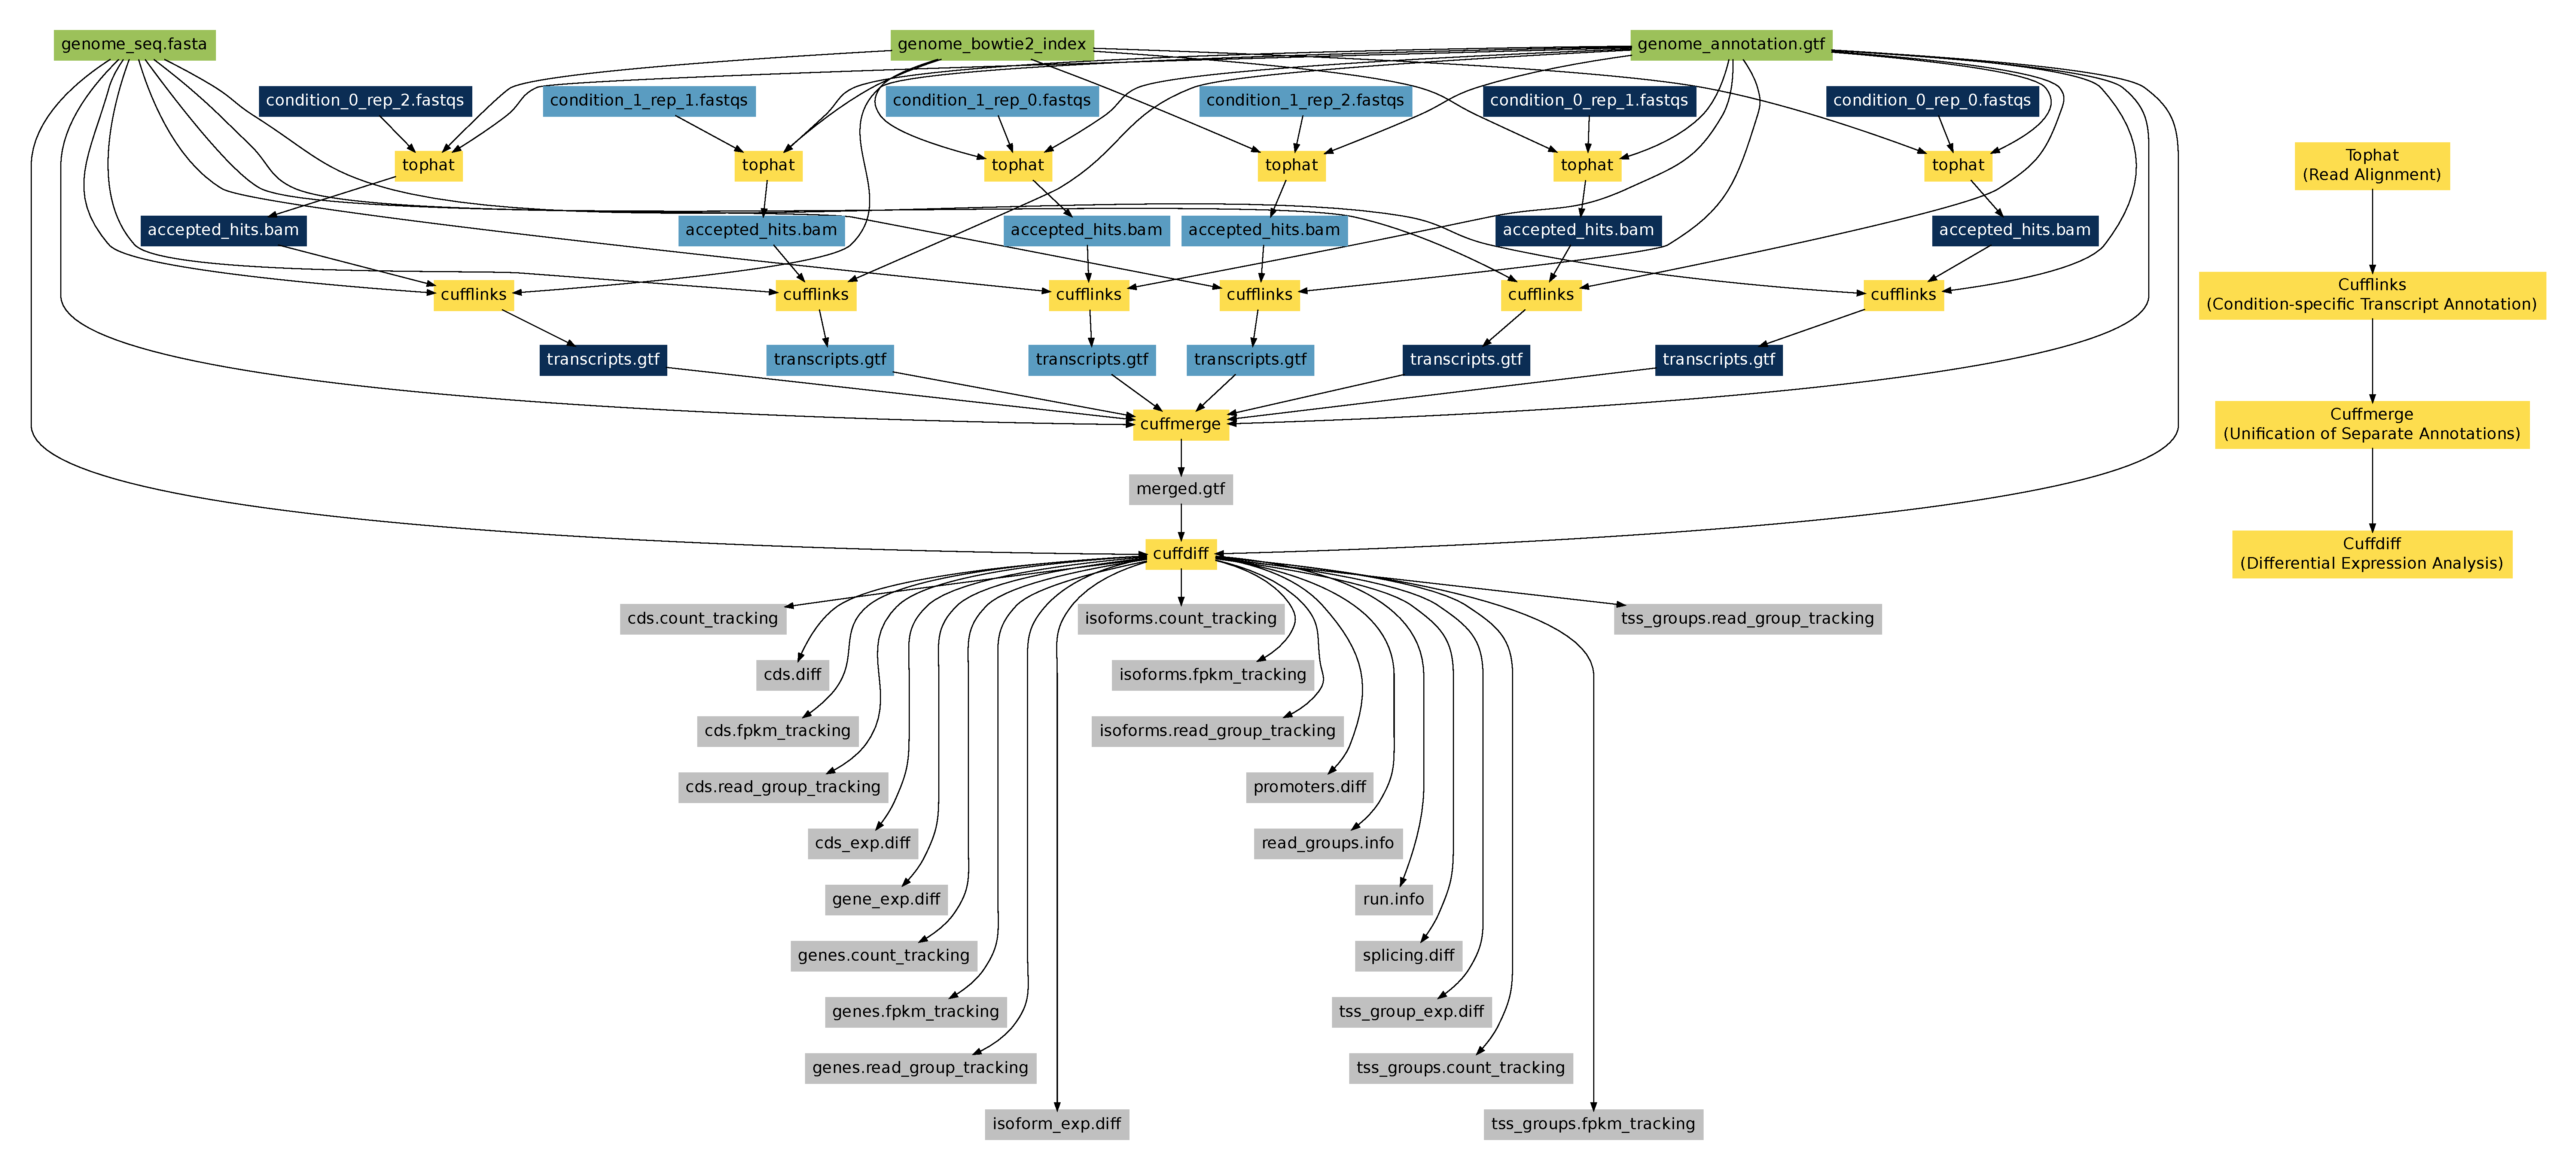
\includegraphics[width=\linewidth]{figures/figs/tuxedo_dot/707354_6/tophat_cufflinks_ins_outs.pdf}
\caption[Diagram of Abbreviated Tophat/Cufflinks Inputs and Outputs]{\sf \textbf{Diagram of Abbreviated Tophat/Cufflinks Inputs and Outputs:}\\
	This figure demonstrates the complexities of a typical RNA-seq experiment as analyzed with the \gls{TuxProt}. It models a fairly \textbf{simple} two condition experiment with each condition having three replications. It is ``abbreviated'' in that it only displays the output files that will be used in the next step for all steps except the \UseVerb{cuffdiff} step. The complete output of \UseVerb{cuffdiff} is included to demonstrate the final challenge of integrating the data which exists in multiple cross-referenced files.\\ 
	(\emph{Dark Blue} - Inputs/Outputs associated with Condition Zero; 
	\emph{Light Blue} - Inputs/Outputs associated with Condition One; 
	\emph{Grey} - Inputs/Outputs associated with Condition Zero \textbf{AND} Condition One; 
	\emph{Green} - Inputs Specific to the Reference Genome; 
	\emph{Gold} - Program Calls)
}
	\label{fig:tuxedo}
\end{figure}
 
 
 
\end{landscape}






%%% Local Variables: ***
%%% mode: latex ***
%%% TeX-master: "thesis.tex" ***
%%% End: ***
